% Settings
\documentclass[a4paper,oneside,12pt]{article}
\usepackage[utf8]{inputenc}
\usepackage[czech]{babel}
\usepackage{graphicx}
\usepackage{mathtools}
\addtolength{\textwidth}{2cm}
\addtolength{\hoffset}{-1cm}
\addtolength{\textheight}{5cm}
\addtolength{\voffset}{-2.5cm}
\DeclareGraphicsExtensions{.pdf,.png,.jpg}
\graphicspath{./images/}
% /Settings

% Description
\author{Syanova Elizaveta (xsyano00)}
\date{\today}
\title{Semestralní projekt IEL}
% /Description

% Content
\begin{document}
	\maketitle
	\tableofcontents
    
	\newpage

	% Section Příklad 1
	\section{Příklad 1}
	\maketitle


	Stanovte napětí $U_{R6}$ a proud $I_{R6}$. Použijte metodu postupného
	zjednodušování obvodu.

	\begin{table}[h]
		\begin{center}
			\begin{tabular}{|c|c|c|c|c|c|c|c|c|c|c|c|c|c|c|}
				\hline
				sk. & $U_{1}$ [$V$] & $U_{2}$ [$V$] & $R_{1}$ [$\Omega$] & $R_{2}$ [$\Omega$] & $R_{3}$ [$\Omega$] & $R_{4}$ [$\Omega$] & $R_{5}$ [$\Omega$] & $R_{6}$ [$\Omega$] & $R_{7}$ [$\Omega$] & $R_{8}$ [$\Omega$] \\
				\hline
				H & 135 & 80 & 680 & 600 & 260 & 310 & 575 & 870 & 355 & 265 \\
				\hline
			\end{tabular}
		\end{center}
	\end{table}

	\begin{figure}[h]
		\begin{center}
			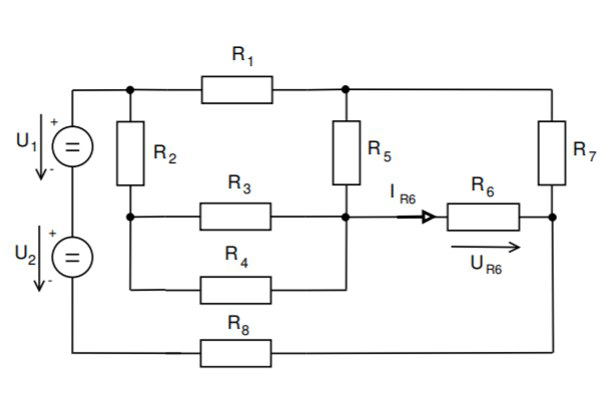
\includegraphics[width=8cm,keepaspectratio]{images/1_img.png}
		\end{center}
	\end{figure}

	Zapojení postupně zjednodušíme:
	\begin{eqnarray*}
		R_{34} &= & \frac{R_{3} * R_{4}}{R_{3} + R_{4}} = \frac{260 * 310}{260 + 310} = 141,4035\Omega\\
		R_{234} &= & R_{2} + R_{34} = 600 + 141,4035 = 741,4035 \Omega\\
	\end{eqnarray*}

	Vzniklý trojúhelník [$R_{4}$, $R_{57}$, $R_{68}$] převedeme na hvězdu:
	\begin{eqnarray*}
		R_{A} &= & \frac{R_{1} * R_{234}}{R_{1} + R_{234} + R_{5}} = \frac{680 * 741,4035}{680 + 741,4035 + 575} = 252,5313 \Omega\\
		R_{B} &= & \frac{R_{1} * R_{5}}{R_{1} + R_{234} + R_{5}} = \frac{680 * 575}{680 + 741,4035 + 575} = 195.8522 \Omega\\
		R_{C} &= & \frac{R_{5} * R_{234}}{R_{1} + R_{234} + R_{5}} = \frac{575 * 741,4035}{680 + 741,4035 + 575} = 213.5375 \Omega\\
	\end{eqnarray*}

	Dále zjednodušíme:
	\begin{eqnarray*}
		R_{B7} &= & R_{B} + R_{7} = 195,8522 + 355 = 550.8522 \Omega\\
		R_{C6} &= & R_{С} + R_{6} = 213.5375 + 870 = 1083.5375 \Omega\\
		R_{B7C6} &= & \frac{R_{B7} * R_{C6}}{R_{B7} + R_{C6}} = \frac{550.8522 * 1083.5375}{550.8522 + 1083.5375} = 365.1938 \Omega\\
		R &= & R_{A} + R_{B7C6} + R_{8} = 252.5313 + 365.1938 + 265 = 882.7251 \Omega\\
	\end{eqnarray*}

	Vypočteme proud zdroje:
	\begin{eqnarray*}
		U &= & U_{1} + U_{2} = 135 + 80 = 215 \Omega\\
		I &= & \frac{U}{R} = \frac{215}{882.7251} = 0.2435 A\\
	\end{eqnarray*}

	Ze získaných hodnot vypočteme hledané hodnoty $I_{R6}$ a $U_{R6}$:
	\begin{eqnarray*}
		U_{RC6} &= & U_{C6B7} = I * R_{C6B7} = 0.2435 * 365.1938 = 88.948 V\\
		I_{R6} &= & I_{RC6} = \frac{U_{RC6}}{R_{C6}} = \frac{88.948}{1083.5375} = 0.082 A\\
		U_{R6} &= & I_{R6} * R_{6} = 0.082 * 870 = 71.35 V\\
	\end{eqnarray*}

	Hledané hodnoty $I_{R6}$ a $U_{R6}$ jsou:
	\begin{eqnarray*}
		I_{R6} &= & 0.082 A\\
		U_{R6} &= & 71.35 V\\
	\end{eqnarray*}

	\newpage

	% Example 2
	\section{Příklad 2}

	Stanovte napětí $U_{R3}$ a proud $I_{R3}$. Použijte metodu Théveninovy věty.

	\begin{table}[h]
		\begin{center}
			\begin{tabular}{|c|c|c|c|c|c|c|c|c|}
				\hline
				sk. & $U$ [$V$] & $R_{1}$ [$\Omega$] & $R_{2}$ [$\Omega$] & $R_{3}$ [$\Omega$] & $R_{4}$ [$\Omega$] & $R_{5}$ [$\Omega$] & $R_{6}$ [$\Omega$]\\
				\hline
				A & 50 & 100 & 525 & 620 & 210 & 530 & 100 \\
				\hline
			\end{tabular}
		\end{center}
	\end{table}

	\begin{figure}[h]
		\begin{center}
			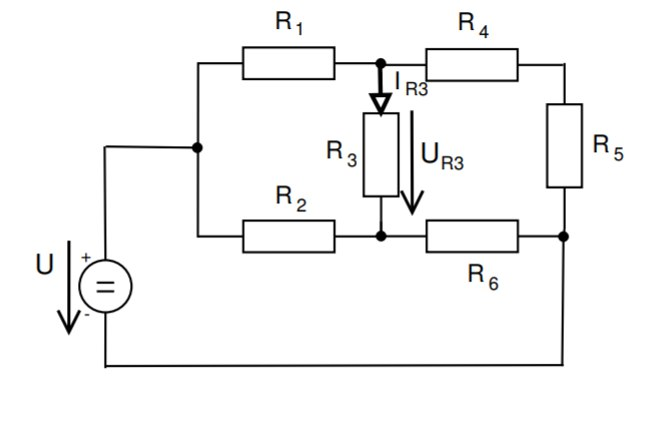
\includegraphics[width=8cm,keepaspectratio]{images/2_img.jpg}
		\end{center}
	\end{figure}

	Zapojení postupně zjednodušíme pro výpočet odporu $R_{i}$:
	\begin{eqnarray*}
		R_{45} &= & R_{4} + R_{5} = 210 + 530 = 740 \Omega\\
		R_{145} &= & R_{1} || R_{45} = \frac{R_{1} * R_{45}}{R_{1} + R_{45}} = \frac{100 * 740}{100 + 740} = 88.0952 \Omega\\
		R_{26} &= & R_{2} || R_{6} = \frac{R_{2} * R_{6}}{R_{2} + R_{6}} = \frac{525 * 100}{525 + 100} = 84 \Omega\\
		R_{i} &= & R_{145} + R_{26} = 88.0952 + 84 = 172.0952 \Omega\\
	\end{eqnarray*}

	Zapojení postupně zjednodušíme pro výpočet napětí $U_{i}$:
	\begin{eqnarray*}
		R_{145} &= & R_{1} + R_{45} = 100 + 740 = 840 \Omega\\
		R_{26} &= & R_{2} + R_{6} = 525 + 100 = 625 \Omega\\
		R_{14526} &= & R_{145} || R_{26} = \frac{R_{145} * R_{26}}{R_{145} + R_{26}} = \frac{840 * 625}{840 + 625} = 358.3617 \Omega\\
	\end{eqnarray*}

	Vypočteme proudy $I_{1}$ pro rezistor $R_{145}$ a $I_{2}$ pro $R_{26}$:
	\begin{eqnarray*}
		I_{1} &= & \frac{U}{R_{145}} = \frac{50}{840} = 0.0595 A\\
		I_{2} &= & \frac{U}{R_{26}} = \frac{50}{625} = 0.08 A\\
	\end{eqnarray*}

	Dle II. Kirchhoffova zákona vypočteme napětí $U_{i}$ ze smyčky tvořené větvemi s rezistory $R_{1}$, $R_{2}$ a $R_{3}$:
	\begin{eqnarray*}
		U_{i} &= & - I_{1} * R_{1} + I_{2} * R_{2} \\
		U_{i} &= & - 0.0595 * 100 + 0.08 * 525 \\
		U_{i} &= & 36.05 V\\
	\end{eqnarray*}

	Ze získaných hodnot vypočteme hledané hodnoty $I_{R3}$ a $U_{R3}$:
	\begin{eqnarray*}
		I_{R3} &= & \frac{U_{i}}{R_{i} + R_{3}} = \frac{36.05}{172.0952 + 620} = 0.0455 A\\
		U_{R3} &= & I_{R3} * R_{3} = 0.0455 * 620 = 28.2175 V\\
	\end{eqnarray*}

	Hledané hodnoty $I_{R3}$ a $U_{R3}$ jsou:
	\begin{eqnarray*}
		I_{R3} &= & 0.0455 A\\
		U_{R3} &= & 28.2175 V\\
	\end{eqnarray*}

	\newpage

	% Example 3
	\section{Příklad 3}

	Stanovte napětí $U_{R2}$ a proud $I_{R2}$. Použijte metodu uzlových napětí ($U_{A}, U_{B}, U_{C}$).

	\begin{table}[h]
		\begin{center}
			\begin{tabular}{|c|c|c|c|c|c|c|c|c|}
				\hline
				sk. & $U$ [$V$] & $I_{1}$ [$A$] & $I_{2}$ [$A$] & $R_{1}$ [$\Omega$] & $R_{2}$ [$\Omega$] & $R_{3}$ [$\Omega$] & $R_{4}$ [$\Omega$] & $R_{5}$ [$\Omega$]\\
				\hline
				C & 110 & 0.85 & 0.75 & 44 & 31 & 56 & 20 & 30 \\
				\hline
			\end{tabular}
		\end{center}
	\end{table}

	\begin{figure}[h]
		\begin{center}
			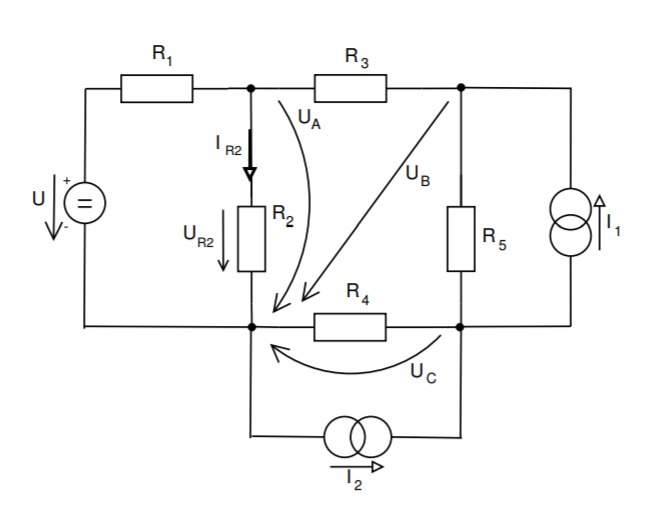
\includegraphics[width=8cm,keepaspectratio]{images/3_img.jpg}
		\end{center}
	\end{figure}

	Dle I. Kirchhoffova zákona sestavíme rovnice pro uzly $A, B, C$:
	\begin{eqnarray*}
		A &: & I_{R1} - I_{R3} - I_{R2} = 0 \\
		B &: & I_{1} + I_{R3} - I_{R5} = 0\\
		C &: & I_{2} - I_{1} + I_{R5} - I_{R4} = 0\\
	\end{eqnarray*}


	Dosadíme jednotlivé proudy do připravených rovnic:
	\begin{eqnarray*}
		0 &= & G_{1}(U - U_{A}) - G_{3}(U_{A} - U_{B}) - G_{2}U_{A}  \\
		0 &= & I_{1} + G_{3}(U_{A} - U_{B}) - G_{5}(U_{B} - U_{c}) \\
		0 &= & I_{2} - I_{1} + G_{5}(U_{B} - U_{C}) - G_{4}U_{C} \\
	\end{eqnarray*}

	Upravíme rovnice:
	\begin{eqnarray*}
		- U_{A}(G_{1} + G_{2} + G_{3}) + U_{B}G_{3} + 0U_{C} & =& - G_{1}U \\
		U_{A}G_{3} - U_{B}(G_{3} + G_{5}) + G_{5}U_{C} & =& - I_{1} \\
		0U_{A} + G_{5}U_{B} - U_{C}(G_{4} + G_{5}) & =& I_{1} - I_{2} \\
	\end{eqnarray*}

	Dosadíme číselné hodnoty:
	\begin{eqnarray*}
	    - U_{A}(\frac{1}{44} + \frac{1}{31} + \frac{1}{56}) + U_{B}\frac{1}{56} + 0U_{C} & =& - \frac{110}{44} \\
	    U_{A}\frac{1}{56} - U_{B}(\frac{1}{56} + \frac{1}{30}) + U_{C}\frac{1}{30} & =& - 0.85 \\
	    0U_{A} + U_{B}\frac{1}{30} - U_{C}(\frac{1}{20} + \frac{1}{30}) & =& 0.85 - 0.75 \\
	\end{eqnarray*}

	Zapíšeme v podobě rozšířené matice, cramerovým pravidlem vypočteme uzlová napětí $U_{A}$:
	\begin{eqnarray*}
		A &= &
			\begin{pmatrix}			
				-0.0727 & 0.0278 & 0 & \vline & -2.5 \\
				0.0178 & -0.0511 & 0.0333 & \vline & -0.85 \\
				0 & 0.0333 & -0.0833 & \vline & 0.1
			\end{pmatrix} \\
		\\
		det A &= &
			\begin{vmatrix}
				-0.0727 & 0.0278 & 0  \\
				0.0178 & -0.0511 & 0.0333 \\
				0 & 0.0333 & -0.0833
			\end{vmatrix} = -2.0199 * 10^{-4} \\
		\\
		U_{A} &= & \frac{
			\begin{vmatrix}
				-2.5 & 0.0278 & 0 \\
				-0.85 & -0.0511 & 0.0333 \\
				0.1 & 0.0333 & -0.0833
			\end{vmatrix}
		}{det A} = \frac{-9.0704 * 10^{-3}}{-2.0199 * 10^{-4}} = 44.9052 V\\
	\end{eqnarray*}

	Ze získaných hodnot vypočteme hledané hodnoty $U_{R3}$ a $I_{R3}$:
	\begin{eqnarray*}
		U_{R2} &= & U_{A} = 44.9052 V\\
		I_{R2} &= & \frac{U_{R2}}{R_{2}} = \frac{44.9052}{31} = 1.4458 A\\
	\end{eqnarray*}

	Hledané hodnoty $U_{R3}$ a $I_{R3}$ jsou:
	\begin{eqnarray*}
		U_{R2} &= & 44.9052 V\\
		I_{R2} &= & 1.4458 A\\
	\end{eqnarray*}

	\newpage

	% Section Závěr
	\section{Závěr}
	\maketitle

	\begin{table}[ht]
		\begin{center}
			\begin{tabular}{|c|c|c|}
				\hline
				Příklad & Zadání & Výsledek \\
				\hline
				1 & H & $U_{R6} = 71.35 V$, $I_{R6} = 0.082 A$ \\
				\hline
				2 & A & $U_{R3} = 28.2175 V$, $I_{R3} = 0.0455 A$ \\
				\hline
				3 & C & $U_{R2} = 44.9052 V$, $I_{R2} = 1.4458 A$ \\
				\hline
				4 & H &   \\
				\hline
				5 & B &  \\
				\hline
			\end{tabular}
			\caption{Výsledky řešení}
		\end{center}
	\end{table}

\end{document}
% /Content

% paralel
% R_{} &= & R_{} || R_{} = \frac{R_{} * R_{}}{R_{} + R_{}} = \frac{ * }{ + } =  \Omega\\

% serial
% R_{} &= & R_{} + R_{} =  +  =  \Omega\\